% Options for packages loaded elsewhere
\PassOptionsToPackage{unicode}{hyperref}
\PassOptionsToPackage{hyphens}{url}
%
\documentclass[
]{article}
\usepackage{lmodern}
\usepackage{amssymb,amsmath}
\usepackage{ifxetex,ifluatex}
\ifnum 0\ifxetex 1\fi\ifluatex 1\fi=0 % if pdftex
  \usepackage[T1]{fontenc}
  \usepackage[utf8]{inputenc}
  \usepackage{textcomp} % provide euro and other symbols
\else % if luatex or xetex
  \usepackage{unicode-math}
  \defaultfontfeatures{Scale=MatchLowercase}
  \defaultfontfeatures[\rmfamily]{Ligatures=TeX,Scale=1}
\fi
% Use upquote if available, for straight quotes in verbatim environments
\IfFileExists{upquote.sty}{\usepackage{upquote}}{}
\IfFileExists{microtype.sty}{% use microtype if available
  \usepackage[]{microtype}
  \UseMicrotypeSet[protrusion]{basicmath} % disable protrusion for tt fonts
}{}
\makeatletter
\@ifundefined{KOMAClassName}{% if non-KOMA class
  \IfFileExists{parskip.sty}{%
    \usepackage{parskip}
  }{% else
    \setlength{\parindent}{0pt}
    \setlength{\parskip}{6pt plus 2pt minus 1pt}}
}{% if KOMA class
  \KOMAoptions{parskip=half}}
\makeatother
\usepackage{xcolor}
\IfFileExists{xurl.sty}{\usepackage{xurl}}{} % add URL line breaks if available
\IfFileExists{bookmark.sty}{\usepackage{bookmark}}{\usepackage{hyperref}}
\hypersetup{
  pdftitle={Child survival for mothers: mortality change and related measures},
  pdfauthor={Iván Williams and Diego Alburez-Gutierrez},
  hidelinks,
  pdfcreator={LaTeX via pandoc}}
\urlstyle{same} % disable monospaced font for URLs
\usepackage[margin=1in]{geometry}
\usepackage{graphicx,grffile}
\makeatletter
\def\maxwidth{\ifdim\Gin@nat@width>\linewidth\linewidth\else\Gin@nat@width\fi}
\def\maxheight{\ifdim\Gin@nat@height>\textheight\textheight\else\Gin@nat@height\fi}
\makeatother
% Scale images if necessary, so that they will not overflow the page
% margins by default, and it is still possible to overwrite the defaults
% using explicit options in \includegraphics[width, height, ...]{}
\setkeys{Gin}{width=\maxwidth,height=\maxheight,keepaspectratio}
% Set default figure placement to htbp
\makeatletter
\def\fps@figure{htbp}
\makeatother
\setlength{\emergencystretch}{3em} % prevent overfull lines
\providecommand{\tightlist}{%
  \setlength{\itemsep}{0pt}\setlength{\parskip}{0pt}}
\setcounter{secnumdepth}{-\maxdimen} % remove section numbering

\title{Child survival for mothers: mortality change and related measures}
\author{Iván Williams and Diego Alburez-Gutierrez}
\date{May 2020}

\begin{document}
\maketitle

\hypertarget{introduction}{%
\subsection{Introduction}\label{introduction}}

The question of child survival for mothers sits at the very center of
demographic theory. Offspring survival is usually studied alongside
fertility decline in the context of the demographic transition, but it
also matters for post-transitional societies. Lower fertility and higer
life expectancy means that fewer children are expected to provide key
emotional, social, and financial transfers to aging parents for longer
periods of time. With increasing periods of generational overlap,
individuals find themselves `sandwiched' between aging parents and young
children requiring their simultaneous attention and care (Daatland,
Veenstra, and Lima 2010). In the context of global population aging,
elderly parents without access to formal social security and pension
systems are particularly reliant on these transfers (Smith-Greenaway and
Trinitapoli 2020). Given the known psychological, health, and social
consequences of child loss for bereaved parents and families
(Hendrickson 2009; Lee et al. 2014), it is surprising that the
demographic processes that shape parental bereavement remain very poorly
understood.

The Covid-19 pandemic has underscored the need to understand how sudden
changes in mortality affect the availability of kin. The elderly depend
on kin support, especially during periods of lockdown and in the absence
of governmental support mechanisms. Elderly mothers may be at a higher
risk of losing the key support provided by their adult children given
the known age-gradient in the Covid-19 case fatality rate. How do
changes in mortality affect the availability of offspring over age from
the point of view of a prospective mother? How do these processes play
out in a heterogeneous population?

In this paper, we aim to formalize the relationship between
population-level changes in mortality rates (additive or multiplicative)
and changes in the lived experience of kin death. This is key for
understanding the impact of age-specific excess mortality on the
resilience or otherwise of kinship networks for the vulnerable elderly
population. This paper uncovers formal relationships and provides
numerical applications using data from Latin America in the second half
of the twentieth century using period measures in a stable
context.\footnote{See the \protect\hyperlink{Applications}{Applications}
  section for more details on the source, calculation procedures and
  main numerical results.} We continue a long tradition in mathematical
demography, starting with the work of Lotka (1931) on modelling
orphanhood in theoretical populations, Brass (1953) on child survival,
Goodman, Keyfitz, and Pullum (1974) on kin survival in stable
populations, and recently, Caswell (2019) kinship matrices.

\hypertarget{relationship-and-proofs}{%
\subsection{Relationship (and proofs)}\label{relationship-and-proofs}}

\hypertarget{child-survival}{%
\subsubsection{Child Survival}\label{child-survival}}

Let \(CS_a\) be the expected number of surviving children to a
mother\footnote{We use woman and mother interchangeably in this paper,
  assuming that all women are exposed to the same fertility rates.}
alive at aged \(a\) in a female stable population with fertility rates
\(m_{x}\), mortality hazard \(\mu_{x}\) and survival function
\(l_x=e^{-\int_{0}^{x}{\mu_t}\,dt}\) (with unit radix \(l_0=1\)), as
proposed by Goodman, Keyfitz, and Pullum (1974):

\[CS_a = \int_{0}^a{m_{x}l_{a-x}dx}\]

\hypertarget{an-approximation}{%
\subsubsection{An approximation}\label{an-approximation}}

As an initial step, we seek an intuitive understanding of the previous
relation. Building on work by Keyfitz and Caswell (2005) for the
probability of a living mother, we can show which features of the child
survival function explain the expected number of children. For this we
use an approximate of \(l_x\) using Taylor´s theorem until second order
around the mean age of childbearing \(\kappa\):

\[
\begin{aligned}
CS_a \approx & l_{a-\kappa} \int_{0}^a{m_{x}dx}+(l_{a-\kappa})^{'}\int_{0}^a{(x-\kappa)m_{x}dx}+
(l_{a-\kappa})^{''}\int_{0}^a{\frac{(x-\kappa)^2}{2} m_{x}dx}\\
  & \approx F_a l_{a-\kappa} + \frac{\sigma^2}{2}F_a (l_{a-\kappa})^{''}\\
  & \approx F_a \, l_{a-\kappa}[1+\frac{\sigma^2}{2}\frac{(l_{a-\kappa})^{''}}{l_{a-\kappa}}]
\end{aligned}
\]

where the fertility pattern by age is concentrated around \(\kappa\) and
the accumulated fertility (or gross reproduction rate in our
female-dominant scenario) is \(F_a = \int_{\alpha}^a{m_{x}dx}\). The
second Taylor´s term is null because
\(\int_{\alpha}^a{x \, m_{x}dx} = \kappa \, F_a\).

We find that, seen from the perspective of a mother, child survival
mainly depends on the cummulative fertility function and the survival of
daughters from birth to \(a-\kappa\). The approximation is affected
negativally by how disperse is the fertility by age (variance
\(\sigma^2\)) and the survival curvature around (with negative sign), in
an age range where \(l_x\) is tipycally very flat in transitioned
populations (range 20-40 years old)\footnote{This approximation is
  useful also for get an idea of impact because of changes in the
  fertility average age \(\kappa\), keeping constant the level: taking
  logs in \(F_a \, l_{a-\kappa}\) and deriving we get
  \(\frac{\Delta CS_a}{CS_a} \approx \mu_{a-\kappa} \Delta\kappa\),
  being daughters exposed to less time beacuse of the delay in pattern}.

\hypertarget{mortality-changes}{%
\subsubsection{Mortality Changes}\label{mortality-changes}}

We now consider the consequences of an absolute change \(\delta\) in
mortality in the range \([0,a-\alpha]\), where \(\alpha\) is the start
age of fertility risk. For now, let us consider
\(m_{x,\delta}=m_{x}+\delta\) (Wrycza and Baudisch (2012)) and
\(l_{a-x}^\delta = e^{-\int_{0}^{a-x}{(\mu_t+\delta})dt}\):

\[CS_{a}^\delta = \int_{\alpha}^{a}m_{x} l_{a-x} e^{-\delta (a-x)} dx\]

We get the derivative of \(dCS_{(a)}^\delta / d\delta\) evaluated near
zero (Keyfitz and Caswell (2005)) to find the effects of adding
\(\delta\) to hazard rates:

\[
\begin{aligned}
\frac{dCS^{\delta}}{d\delta} = -a\int_{\alpha}^{a}m_{x}{l_{a-x} dx} + \int_{\alpha}^{a} x m_{x} {l_{a-x} dx}\\
= -a \, CS_{a}  + \int_{\alpha}^{a} {x  \, m_{x} l_{a-x} dx}
\end{aligned}
\]

Dividing both sides by \(CS_{a}\) in an discrete approximation we get:

\[\frac{\Delta CS_{a}}{CS_{a}} \approx -(a - k_a) \Delta\delta\]

The expected change in descendants survival is inversely proportional to
the difference between maternal age \(a\) and the mean age of the mother
at the birth of her surviving daughters \(k_a\). The magnitude of the
change depends negatively on the age distribution of the surviving
offspring (the younger the fertility bigger the impact), which is
intuitive considering that older descendants experiences longer periods
of exposure to risk.

However, it is unlikely for mortality to change at the same rate at all
ages. In the course of the demographic transition, for example, we would
expect larger changes in young-age mortality. Consider a change in
infant mortality in the age range \(\left[0;1\right)\). We can inspect
the effect in child survival \(CS_{a}^{\delta_0}\) by splitting the
integral between those daughters who were exposed to the mortality
change and those who were not (now generalizing for \(\alpha\) positive
and \(a>1\) for simplicity):

\[
\begin{aligned}
CS_{a}^{\delta_0} = \int_{0}^{a-1} m_{x} {e{^{-\int_{1}^{a-x}\mu_t \,dt-\int_{0}^{1}(\mu_t + \delta)\,dt}}} dx + \int_{a-1}^{a} m_{x} e^{-\int_{0}^{a-x}(\mu_t+ \delta)\,dt}dx \\
=\int_{0}^{a-1} m_{x} l_{a-x}e^{-\delta} dx + \int_{a-1}^{a} m_{x} l_{a-x} e^{-\delta(a-x)}\,dx
\end{aligned}
\] Deriving by \(\delta\) and valuating near 0, we get:

\[\frac{dCS^{\delta_0}}{d\delta_0} =-\int_{0}^{a-1} m_{x} l_{a-x} dx - a \int_{a-1}^{a} {m_{x} l_{a-x} dx} + \int_{a-1}^{a} {x \, m_{x} l_{a-x} dx}\]
Given that \(CS_{a-1,a}=\int_{a-1}^{a} {m_{x} l_{a-x} dx}\), we can
express the first term in the right as \(CS_a - CS_{a-1,a}\). The
righ-most term could also be expressed as \(\kappa_{a-1,a} CS_{a-1,a}\),
so that:

\[ \frac{dCS^{\delta_0}}{d\delta_0} = - CS_a + CS_{a-1,a} (1-a+\kappa_{a-1,a})\]
The factor \(1-(a-\kappa_{a-1,a})\), which lies between 0 and 1, is
equal to the average portion of time spent with living daughters durings
age \emph{a}. Assuming a uniform distribution of those births,
discretizing the change and dividing by \(CS_a\) we get the final
expression for change in infant mortality:

\[\frac{\Delta CS_{a}^{\delta_0}}{CS_{a}} \approx - \left[1-\frac{CS_{a-1,a}}{CS_a}\frac{1}{2}\right] \Delta\delta\]

This means that an absolute change in infant hazard rate affects
proportionally for all the age range extension (cohorts aged more than
1), except for ``half'' the portion \(\frac{CS_{a-1,a}}{CS_a}\) on how
important was this las age in total ``successful'' experience (in terms
of alive descendants). If \(a\) is near \(\beta\) then
\(\frac{\Delta CS_{a}^{\delta_0}}{CS_{a}} \approx -\Delta\delta\).

We now consider the consequences of a proportional change in mortality
on child survival. Given a proportional change in mortality
\(\mu_{x,\delta}=\mu_{x}(1+\delta)\) so that
\(l_{a-x}^\delta = e^{-\int_{0}^{a-x}{\mu_t(1+\delta})dt}=(l_{a-x})^{(1+\delta)}\),
it follows that:

\[CS_{a}^\delta = \int_{\alpha}^{a} {m_{x} l_{a-x}^{(1+\delta)}} dx.\]

Using the derivative
\(\frac{dl_{a-x}^{(1+\delta)}}{d\delta} = log(l_{a-x}) l_{a-x}^{(1+\delta)}\),
and in the third row reversing integrals between \(t\) and \(x\):

\[
\begin{aligned}
\frac{d CS_{a}^\delta}{d \delta} = \int_{0}^{a} {m_{x} l_{a-x} \log(l_{a-x}) dx}\\
= - \int_{0}^{a} {m_{x} l_{a-x} \int_{0}^{a-x}{\mu_t \, dt}\, dx}\\
= - \int_{0}^{a}{\mu_t} \int_{0}^{a-t} {m_{x} l_{a-t-x} \, dx}\, dt
\end{aligned}
\]

Considering that the last integral is equal to \(CS_{a-t}\), we divide
by \(CS_a\) and multiply by \(\delta\) to obtain:

\[\frac{\Delta CS_{a}}{CS_a} \approx - \left[\int_{0}^{a}{\mu_x  \, \frac{CS_{a-x}}{CS_a} \,dx \,}\right] \Delta \delta\]

This is the negative of cumulative hazard \(H_a\) but considering a
positive factor \(\frac{CS_{a-t}}{CS_a}\) that takes in account the
relative amount of surviving descendants that would be lost at each
child age at risk, that gives more weight to first ages because all the
parity was exposed in that age.

Grasping this relationship intuitively is more difficult given the
interaction of birth and mortality rates (Keyfitz and Caswell (2005)).
The factor \(\frac{CS_{a-t}}{CS_a}\) has a S-shape because \(l_x\)
curvature and fertility accumulation. Taking the difference between
consecutive ages \(a\) and \(a+1\), we have
\(CS_{a-1}=\int_{0}^{a-1} {m_{x} l_{a-1} \, dx}\),
\(CS_{a}=\int_{0}^{a-1} {m_{x} l_{a} \, dx}+CS_{a-1,a}\). In the last
one, a second term is added because of additional born daughters after
\(a-1\), and in the first term the existing one are survived at on
\(\frac{l_{a-x}}{l_{a-1-x}}\). In advanced ages when fertility is
complete, the difference is only explained by the surviving part, that
is why this factor is not a strictly increasing function but for mother
ages close to \(\beta\) (last theoretical fecundity age). We provide a
numerical evaluation of both analytical expressions (absolute an
relative) in the \protect\hyperlink{Applications}{Applications} section.

\hypertarget{related-measures}{%
\subsection{Related Measures}\label{related-measures}}

\hypertarget{burden-and-timing-of-maternal-bereavement}{%
\subsubsection{Burden and timing of maternal
bereavement}\label{burden-and-timing-of-maternal-bereavement}}

We call \emph{Mean Time Spent in Bereavement} (\emph{MTSB}) the absolute
measure of the expected total lifetime with a death daughter for a
mother aged \emph{a}, which can be expressed in terms of a temporary
expected lost years index, in line with \(e^\dagger\) (Vaupel (1986)):

\[MTSB_a = \int_0^a{m_x\int_0^{a-x}{d_t e_{0|a-x-t}\, dt}\,dx} = \int_\alpha^a{m_x e_{0|a-x}^\dagger \,dx}\].

Where \(d_t\) is the death distribution from birth, \(e_{0|a-x-t}\) is
the life expectancy at birth until age \(a-x-t\) and
\(e_{0|a-x}^\dagger\) the temporary dispersion measure. But most
interesting would be to compare these years with the time that mothers
would expect to live with their daughters. We call this the
\emph{Intensity Time in Bereavement} (\(ITB\)): a ratio between expected
time with a ``lost'' and expected time with a ``life'', that allows to
make comparisons between population regimes.

\[ITL_a = \frac{\int_0^a{m_x e_{0|{a-x}}^\dagger dx}}{\int_0^a{m_x e_{0|a-x} dx}}\]

This is a ratio between child-years in two radically different states.
Looks similar to the transcendental entropy measure \(H\) (Keyfitz and
Caswell (2005)) but considering all the cohorts born during the mother´s
life, weighted by their relative size \(m_x\). In the figure
@ref(fig:plot\_ITL\_MAL) is shown that \emph{ITB} is bigger for young
women because of the weight of infant mortality in their mother
experience, also with more dispersion for same levels of parity.

Another important factor for the child survival experience of mothers,
is the mean age at child loss, called here \(MAL\). This relation can be
derived by starting with the mother age \(x+t\) at each death child age
\(t\) at death, weighted by the fertility and survival function. In it,
\(\kappa\) is the mean age at childbirth for women aged \(a\),
\(MAD_{a-x}\) refers to the mean age at death for newborns that die
before \(a-x\) and \(F_a\) is the accumulated fertility for a women aged
\(a\):

\[
\begin{aligned}
MAL_a = & \frac{\int_0^a{m_x {\frac{\int_0^{a-x} l_t \, \mu_t (x+t) dt}{\int_0^{a-x} l_t \, \mu_t dt}}dx}}{\int_0^a{m_x}dx} \\
  MAL_a = & \frac{\int_0^a{m_x \left[{x+\frac{\int_0^{a-x} l_t \, \mu_t \, t \, dt}{\int_0^{a-x} l_t \, \mu_t dt}}\right]dx}}{\int_0^a{m_x}} \\
  MAL_a = & \frac{\int_0^a{m_x \,x \,dx}}{F_a} + \frac{\int_0^a{m_x MAD_{a-x}dx}}{F_a} \\
  MAL_a = & \kappa + \frac{\int_0^a{m_x MAD_{a-x}dx}}{F_a}
\end{aligned}
\]

Following this, in populations with high infant mortality
\(MAD_{a-x}<1\) for all \emph{x}, so \(MAL_a\approx\kappa_a+f_0\), being
\(f_0\) the average time spent for those child that dies in their first
year of life. A numerical approximation of both measures are done in
\protect\hyperlink{Applications}{Applications} section.

\hypertarget{heterogeneity-first-ideas}{%
\subsubsection{Heterogeneity (first
ideas)}\label{heterogeneity-first-ideas}}

In a model with heterogeneity, determined at birth by a multiplicative
effect, \(CS_a\) could be interpreted as a conditional expectation with
random variables \emph{K} for fertility heterogeneity and \emph{Z} for
mortality frailty.

\[CS_a(k,z) = \int_{0}^{\infty}\,{m(k)}_x\,{l(z)}_{a-x}\,dx\]

Following Coresh and Goldman (1988) we can express the fertility part in
a multiplicative way with variability in the level but not in the shape,
as \({m(k)}_x = F_\beta\,k\,r_x\), where \(F_\beta\) is the baseline
cumulated fertility until upper limit in all age range until \(\beta\),
\(k\) is a random variable with mean 1 that allows variability between
groups and \(r_x\) is the fertility structure by age
(\(\int_{0}^{\beta}{r_x}=1\)). In the other side, frailty part can be
thought in a cohort effect way, also in the multiplicative assumption as
Vaupel and Missov (2014), with \(l(z)_x=e^{-H_{x}z}=l_x^z\), with
baseline hazard \(\mu\). Considering the joint distribution \(f_{kz}\),
the intuition could be expressed as \(f_{zk}=f_{k|z}f_z\): groups with
higher descendant´s mortality would adjust their fertility level, with
positive correlation. Replacing both variables, the unconditional mean
\(\overline{CS}_a\) would be\footnote{Note that given k and z values,
  fertility and child survival are independent.}:

\[
\begin{aligned}
\overline{CS}_a = \int_{0}^{\infty}\int_{0}^{\infty}\left[\int_{0}^{a}{ {m(k)}_x l(z)_{a-x}\,dx}\right]f_{kz}\,dz \,dk\\
= F_\beta \int_{0}^{a-x} r_x \int_{0}^{\infty} \int_{0}^{\infty} {(l_{a-x})^z} \, k\, f_{kz} \,dk\,dz\,dx
\end{aligned}
\]

Isolating for an age \emph{x} we can inspect the part related to z and
k: \((l_{a-x})^z \, k\, f_{kz}\). Following Gupta (2018), one way to
create a correlated bivariate distribution is assume for example that
\(Z = Y_0 + Y_1\) and \(K = e^{(Y_0 + Y_2)}\), given the fact that the
historical relation is not linear between both components (see figure
@ref(fig:plot\_tfr\_q0), a funtion \emph{f} like
\(F_\beta=f(ln(q_{0,5}))\). The auxiliar variables \(Y_0\), \(Y_1\) and
\(Y_2\) are independet and Gamma distribuited. Then we can express,
using Laplace transform properties:

\[
\begin{aligned}
\int_{0}^{\infty} \int_{0}^{\infty} {(l_{a-x})^z \, k\, f_{kz} \,dk\,dz}\\
\int_{0}^{\infty} \int_{0}^{\infty}{e^{-H_x(Y_0 + Y_1)}e^{Y_0 + Y_2}}\\
L_{Y_0}[1-H_x]L_{Y_1}[-H_x]L_{Y_2}\,dY_0\,dY_1\,dY_2
\end{aligned}
\]

To continue\ldots{}

\hypertarget{Applications}{%
\subsection{Applications}\label{Applications}}

\hypertarget{Data}{%
\subsubsection{Data}\label{Data}}

We motivate this paper with an empirical example using fertility and
mortality rates from the 2019 Revision of the UN World Population
Prospects (UN WPP) for the Latin American Region (Nations (2019)). We
smoothed female \(l_x\) in quinquennial ages, using cubic-splines
constrained to monotonic decrease, taking \(L_0\) and \(T_{100}\) from
raw life tables as inputs for year-person calculations. For splitting
fertility five groups was used quadratic optimization approach by
Michalski and Gorlishchev (2018), with an desirable property for our
purpose which is a good fitting in parity. Also was assumed an unique
female percentage of newborns of 0.49 for all period-country cases.
Calculations were done in a discrete way assuming that the \(m_x\) live
births are born at exact mother´s age \emph{x}. An already known log
relation between infant mortality and TFR is shown in Latinoamerican
experience (@ref(fig:plot\_tfr\_q0)).

\begin{figure}
\centering
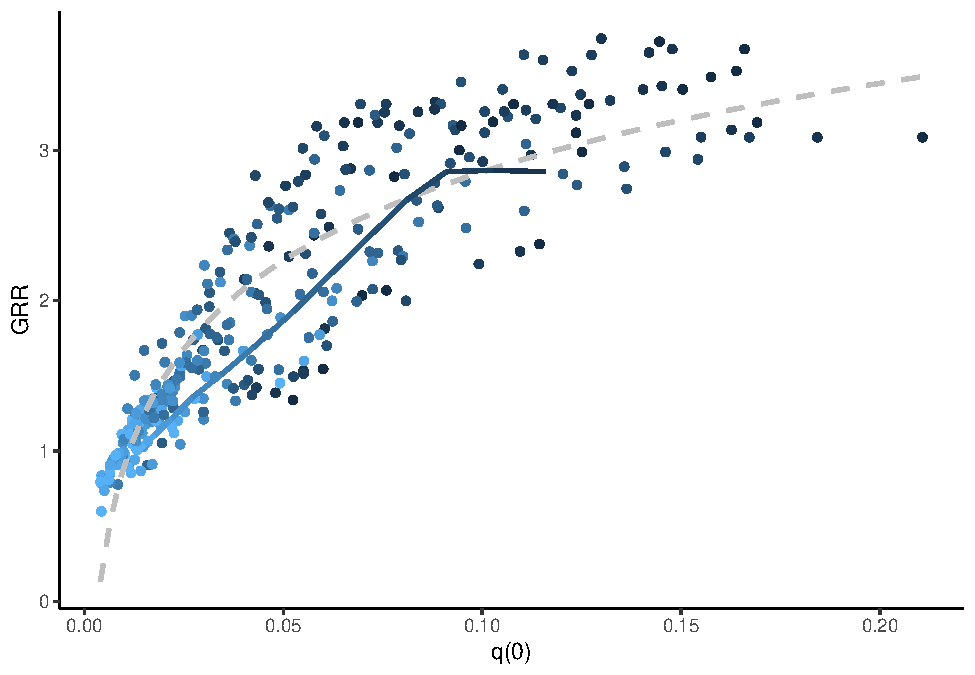
\includegraphics{paper_files/figure-latex/plot_tfr_q0-1.pdf}
\caption{Female probability of death at birth by gross reproduction
rate. Latin America countries in period 1950-2015}
\end{figure}

\hypertarget{numerical-results}{%
\subsubsection{Numerical Results}\label{numerical-results}}

Consider a Latin American woman standing before us. If this were
1950-1955, she could reasonable expect to have 2.23 surviving daughters
on her 50\(^{th}\) birthday. In 2010-2015 a woman the same age would
only have 1.1 living children. The difference of 1.13 children is
explained by reduced fertility and improved mortality in the region
{[}give stats{]}. We now remove the effect of changing fertility by
considering the number of daughters surviving up to maternal age \(a\)
as a proportion of the daughters ever born to a woman that age,
\(\frac{CS_a}{F_a}\). Given Eq. \ref{eq:CS}, the increase from 0.78 in
1950-1955 to 0.97 in 2010-2015 must be explained by a change in
mortality.

\begin{figure}
\centering
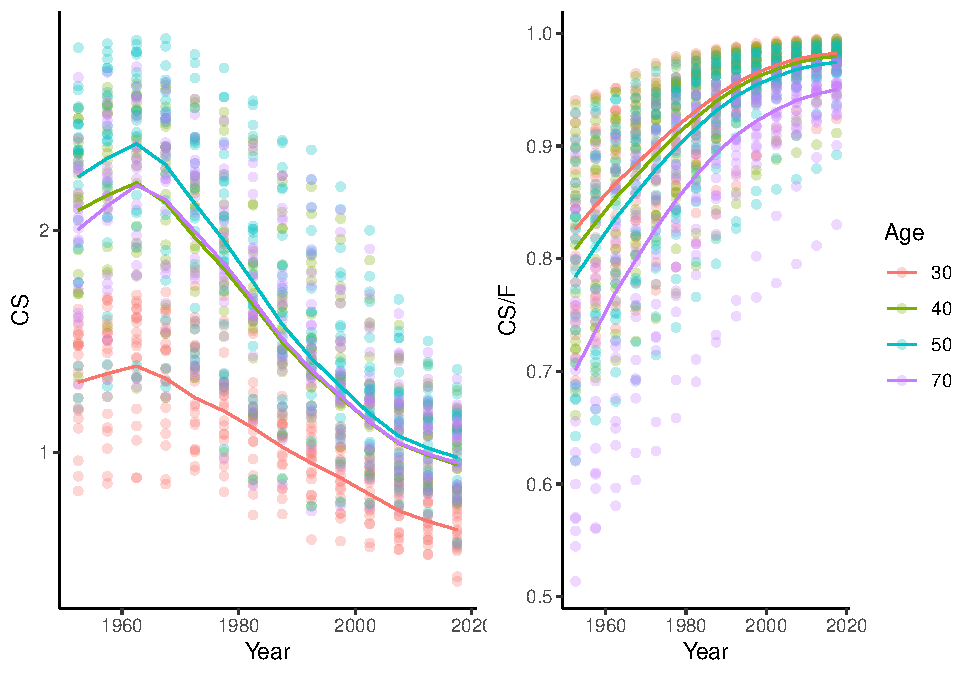
\includegraphics{paper_files/figure-latex/plot_CS-1.pdf}
\caption{Child Survival and Child survival as a share of cummulative
fertility by age, for women aged 30, 40 and 50. Estimates using UN WPP
data for Latin American countries in the period 1950-2015 period}
\end{figure}

The approximation proposed for CS\_a is realy precise, especially for
recent periods. For example, Guatemala improved the approximation with
years due to rectangularization process in \(l_x\) (figure
@ref(fig:plot\_CS\_aprox)).

\begin{figure}
\centering
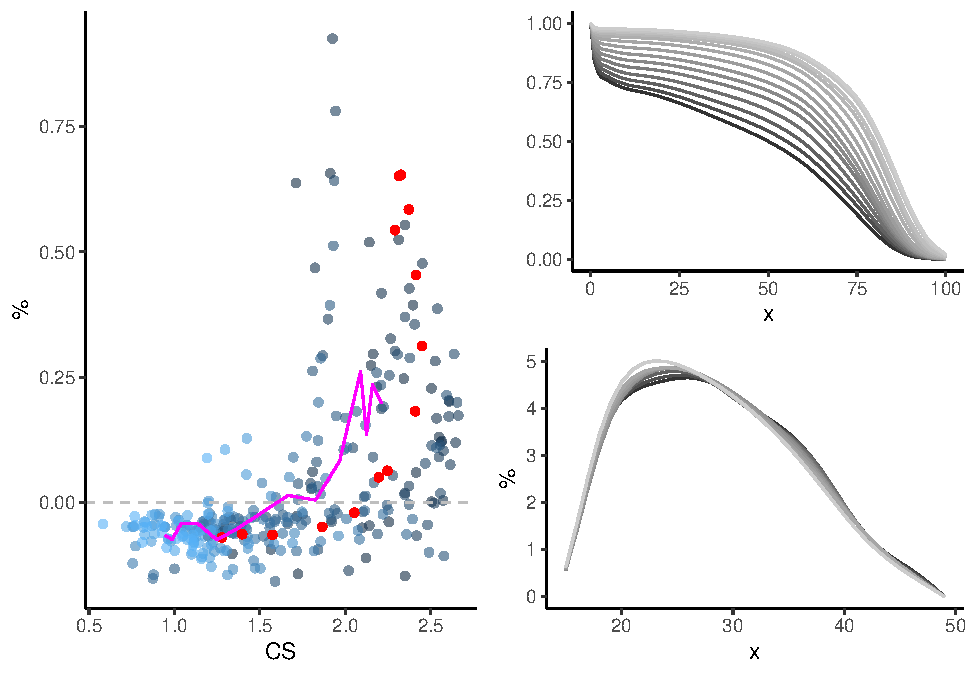
\includegraphics{paper_files/figure-latex/plot_CS_aprox-1.pdf}
\caption{Left: Error in approximation for a=40, from years 1950 (darker)
to 2015 (lighter) for all Latin American countries (blue) and Guatemala
(red). Right: Change in survival and fertility by age in Guatemala.}
\end{figure}

The figure @ref(fig:CS\_abs\_app) shows that goodness of fit is
decreasing with the change size, given that \(\delta\) is assumed near
zero. To ilustrate that considering \(\delta=0.01\) means at age 50, it
means for the absolute change case that
\(\frac{l_{50}}{e^{\delta\,50}} = l_{50}/\) 1.6, a big change). For the
relative case was assumed a constant within each interval
\(\mu_{x+t}=\mu_x\) for \(t\) between 0 and 1,
\(\int_{x}^{x+1}{\mu_t dt} = \log(l_{x+1})-\log(l_{x})\), and was used
this approximation on the empirical data
\(\frac{\Delta CS_{a}}{CS_a} \approx - \left[\sum_{0}^{a-1}{[\log(l_{x+1})-\log(l_{x})]\, \frac{CS_{a-1-x}}{CS_a}\,}\right] \Delta \delta\).

\begin{figure}
\centering
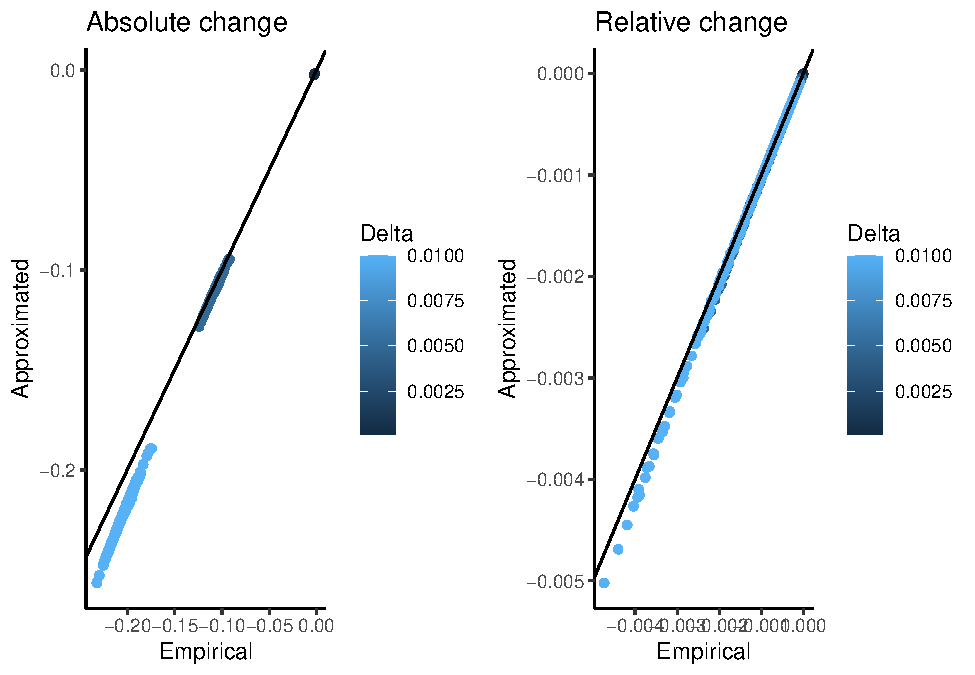
\includegraphics{paper_files/figure-latex/CS_abs_app-1.pdf}
\caption{Effect of absolute and relative change in mortality on child
survival by maternal age of women in Latin America for the 1950-2015
period. Goodness of fit of approximation compared to direct estimation}
\end{figure}

\emph{More develop here showing the factor and ggplot type\ldots{}}

Assuming constant period rates the expected time in years that a mother
aged 30 passed with a death son was around 4\% in some countries at
middle XX Century. When increasing age, the survival experience depends
less on infant mortality, and the distribution is around less than 2\%
for women aged 50, converging to 0 on time. As extreme cases, in
1950-1955 Haiti women aged 30 would have experienced an intensity of
4.8\%, and in 2010-2015 1.4\%, while the women of Costa Rica 2.3\%, and
in 2010-2015 0.2\%. For those Latin American mothers aged 50 with 3
daughters born who suffered a lost, they experienced that at age 30 in
average (figure @ref(fig:plot\_ITL\_MAL)).

\begin{figure}
\centering
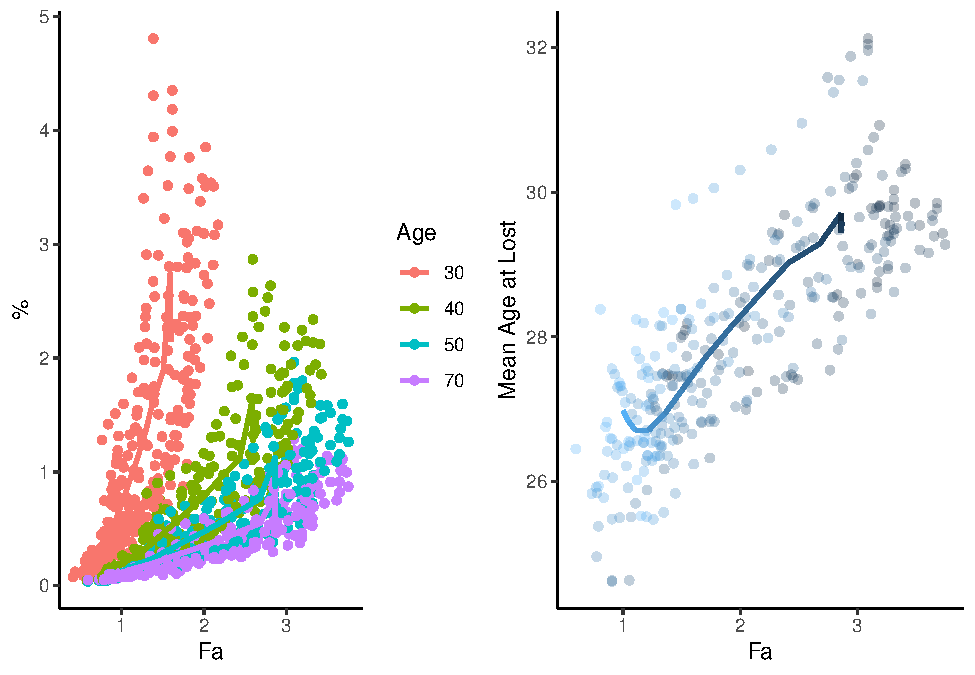
\includegraphics{paper_files/figure-latex/plot_ITL_MAL-1.pdf}
\caption{a) Intensity Tome Lost of women aged 30, 40 and 50. b) Mean age
at Lost for women aged 40. Years 1950 (darker) to 2015 (lighter).
Latinamerican countries in period 1950-2015}
\end{figure}

\hypertarget{references}{%
\subsection*{References}\label{references}}
\addcontentsline{toc}{subsection}{References}

\hypertarget{refs}{}
\leavevmode\hypertarget{ref-brass_derivation_1953}{}%
Brass, W. 1953. ``The Derivation of Fertility and Reproduction Rates
from Restricted Data on Reproductive Histories.'' \emph{Population
Studies} 7 (2): 137. \url{https://doi.org/10.2307/2172029}.

\leavevmode\hypertarget{ref-caswell_formal_2019}{}%
Caswell, Hal. 2019. ``The Formal Demography of Kinship: A Matrix
Formulation.'' \emph{Demographic Research} 41 (September): 679--712.
\url{https://doi.org/10.4054/DemRes.2019.41.24}.

\leavevmode\hypertarget{ref-Coresh1988}{}%
Coresh, Josef, and Noreen Goldman. 1988. ``The effect of variability in
the fertility schedule on numbers of kin.'' \emph{Math. Popul. Stud.} 1
(2): 137--56. \url{https://doi.org/10.1080/08898488809525268}.

\leavevmode\hypertarget{ref-daatland_norwegian_2010}{}%
Daatland, Svein Olav, Marijke Veenstra, and Ivar A. Lima. 2010.
``Norwegian Sandwiches: On the Prevalence and Consequences of Family and
Work Role Squeezes over the Life Course.'' \emph{European Journal of
Ageing} 7 (4): 271--81. \url{https://doi.org/10.1007/s10433-010-0163-3}.

\leavevmode\hypertarget{ref-goodman1974}{}%
Goodman, Leo A, Nathan Keyfitz, and Thomas W Pullum. 1974. ``Family
Formation and the Frequency of Various Kinship Relationships.''
\emph{Theoretical Population Biology} 5 (1): 1--27.

\leavevmode\hypertarget{ref-Gupta2018}{}%
Gupta, R. C. 2018. ``Association measures in the bivariate correlated
frailty model.'' \emph{ResearchGate} 16 (2): 257--78.

\leavevmode\hypertarget{ref-Hendrickson2009}{}%
Hendrickson, K. C. 2009. ``Morbidity, Mortality, and Parental Grief: A
Review of the Literature on the Relationship Between the Death of a
Child and the Subsequent Health of Parents.'' \emph{Palliat Support
Care} 7 (1): 109--19.

\leavevmode\hypertarget{ref-KeyfitzMath}{}%
Keyfitz, Nathan, and Hal Caswell. 2005. \emph{Applied Mathematical
Demography}. Vol. 47. Springer.

\leavevmode\hypertarget{ref-lee_death_2014}{}%
Lee, Chioun, Dana A. Glei, Maxine Weinstein, and Noreen Goldman. 2014.
``Death of a Child and Parental Wellbeing in Old Age: Evidence from
Taiwan.'' \emph{Social Science \& Medicine} 101 (January): 166--73.
\url{https://doi.org/10.1016/j.socscimed.2013.08.007}.

\leavevmode\hypertarget{ref-lotka1931orphanhood}{}%
Lotka, Alfred J. 1931. ``Orphanhood in Relation to Demographic
Factors.'' \emph{Metron} 9 (2): 37--109.

\leavevmode\hypertarget{ref-Michalski2018}{}%
Michalski, Grigoriev, Anatoli I, and Vasily P and Gorlishchev. 2018. ``R
Programs for Splitting Abridged Fertility Data into a Fine Grid of Ages
Using the Quadratic Optimization Method.'' Max Planck Institute for
Demographic Research, Rostock, Germany.

\leavevmode\hypertarget{ref-WPP19}{}%
Nations, United. 2019. \emph{World Population Prospects 2019: Data
Booklet}.
\url{https://doi.org/https://doi.org/https://doi.org/10.18356/3e9d869f-en}.

\leavevmode\hypertarget{ref-smith-greenaway_maternal_2020}{}%
Smith-Greenaway, Emily, and Jenny Trinitapoli. 2020. ``Maternal
Cumulative Prevalence Measures of Child Mortality Show Heavy Burden in
Sub-Saharan Africa.'' \emph{Proceedings of the National Academy of
Sciences}, February, 201907343.
\url{https://doi.org/10.1073/pnas.1907343117}.

\leavevmode\hypertarget{ref-Vaupel2014}{}%
Vaupel, James W., and Trifon I. Missov. 2014. ``Unobserved population
heterogeneity: A review of formal relationships.'' \emph{Demographic
Research} 31 (September): 659--86.
\url{https://www.demographic-research.org/Volumes/Vol31/22}.

\leavevmode\hypertarget{ref-Vaupel1986}{}%
Vaupel, J. W. 1986. ``How Change in Age-Specific Mortality Affects Life
Expectancy.'' \emph{Population Studies} 40 (1): 147--57.
\url{https://doi.org/10.2307/2174285}.

\leavevmode\hypertarget{ref-wrycza2012}{}%
Wrycza, Tomasz, and Annette Baudisch. 2012. ``How Life Expectancy Varies
with Perturbations in Age-Specific Mortality.'' \emph{Demographic
Research} 27: 365--76.

\end{document}
